\documentclass{beamer}
\usepackage[utf8]{inputenc}
\usepackage{textpos} 
\usepackage{graphicx} 
\graphicspath{{./}{DPR_tex/}}
\usepackage{wrapfig}
\usepackage{tikz}
\usetikzlibrary{shapes.geometric,calc, arrows.meta, positioning,fit,backgrounds}
\usepackage{amsmath}
\usepackage{amssymb}
\usepackage[framemethod=TikZ]{mdframed}
\usepackage{caption} 
\usetheme{Boadilla}
\usecolortheme{default}
\usepackage{lmodern}


\usepackage{array}
\usepackage{pgfgantt}
\usepackage{pgf-umlsd}
\usepackage{listings}
\usepackage{adjustbox}
\hfuzz=3pt

\tikzstyle{actor} = [draw, ellipse, minimum height=1.5em, minimum width=3em, align=center]
\tikzstyle{usecase} = [draw, ellipse, minimum height=2.5em, text centered]

% --- PERT NODE PREAMBLE ---
\newcommand{\pertnode}[6]{%
    \node[draw, thick, minimum width=2cm, minimum height=1.15cm,
          fill=white, inner sep=0pt, outer sep=2pt, #2] (#1) at #3 {};%
    \node[font=\scriptsize\bfseries, anchor=center]
          at ([yshift=0.18cm]#1.center) {#4};%
    \draw[thick] ([yshift=-0.08cm]#1.west) -- ([yshift=-0.08cm]#1.east);%
    \draw[thick] ([yshift=-0.08cm]#1.center) -- (#1.south);%
    \node[font=\tiny, anchor=center]
          at ([xshift=-0.5cm, yshift=-0.36cm]#1.center) {#5};%
    \node[font=\tiny, anchor=center]
          at ([xshift=0.5cm, yshift=-0.36cm]#1.center) {#6};%
}
\setbeamertemplate{caption}[numbered]
\renewcommand{\listfigurename}{List of Figures}
\makeatletter
\@ifundefined{tf@lof}{\newwrite\tf@lof}{}
\immediate\openout\tf@lof=\jobname.lof\relax
\newcommand{\storedfigurelist}{}
\newcommand{\figurelistentry}[3]{%
  \g@addto@macro\storedfigurelist{\noindent \textbf{Figure #1.} #2 \dotfill #3\par}%
}
\newcommand{\recordfigureentry}[1]{%
  \protected@write\@auxout{}{\string\figurelistentry{\thefigure}{#1}{\thepage}}%
}
\newcommand{\dynamiclistoffigures}{%
  \begingroup
  \parindent=0pt
  \parskip=0.35em
  \footnotesize
  \ifx\storedfigurelist\@empty
    \textit{No figures listed yet.}%
  \else
    \storedfigurelist
  \fi
  \endgroup
}
\makeatother

\newcommand{\slidepurpose}[2]{%
\vspace*{-0.23cm}
\begin{center}
{\tiny
\setlength{\fboxsep}{3pt}%
\setlength{\fboxrule}{0.6pt}%
\fcolorbox{black!55}{gray!10}{%
\parbox{\dimexpr0.97\linewidth-2\fboxsep-2\fboxrule\relax}{\raggedright
\textbf{Role:} #1 \hfill \textbf{Project Stage:} #2}}}
\end{center}
\vspace{0.03cm}
}
\newcommand{\defitem}[2]{\textbf{#1}: #2\par\vspace{0.32em}}
\newcommand{\solutionfigure}[2]{%
\begin{center}
\begin{minipage}[c][0.72\textheight][c]{\linewidth}
\centering
\includegraphics[width=0.98\linewidth,height=0.68\textheight,keepaspectratio]{#1}
\end{minipage}
\vspace{0.06cm}
{\captionsetup{type=figure,font=tiny,justification=centering}
\captionof{figure}{#2}%
\addcontentsline{lof}{figure}{\protect\numberline{\thefigure}{#2}}%
\recordfigureentry{#2}}
\end{center}
}
\newcommand{\tikzsolutionfigure}[2]{%
\begin{center}
\begin{minipage}[c][0.65\textheight][c]{\linewidth}
\centering
\begin{adjustbox}{max width=0.96\linewidth, max height=0.64\textheight}
#1
\end{adjustbox}
\end{minipage}
\vspace{0.06cm}
{\captionsetup{type=figure,font=tiny,justification=centering}
\captionof{figure}{#2}%
\addcontentsline{lof}{figure}{\protect\numberline{\thefigure}{#2}}%
\recordfigureentry{#2}}
\end{center}
}

\title[Summer Internship Presentation] 
{OpenStack RCA Copilot\\Root Cause Analysis for Cloud Infrastructure}

\subtitle{Design, Evidence Pipeline and Development.}

\author[HANFAOUI Karim] 
{HANFAOUI Karim\inst{1}}

\institute[Huawei Cloud Team] 
{
  \inst{1} EMSI, 4th Year IA \& DATA -- Summer Internship @ Huawei  \\
  Supervisor: HINGER Anass\\
  Karim.Hanfaoui@emsi-edu.ma
}

\date[JUL 2026] 
{Huawei , Casablanca, July 2026}
\titlegraphic{
    \begin{textblock*}{2cm}(8cm, -7.4cm) 
        
\includegraphics[height=0.7cm]{logo} 
    \end{textblock*}
    \begin{textblock*}{2cm}(0cm, -7.7cm) 
        
\includegraphics[height=1.2cm]{huaweii} 
    \end{textblock*}
}
\AtBeginSection[]{}

\begin{document}

\begin{frame}
    \titlepage
\end{frame}

\begin{frame}
\frametitle{Table of Contents}
\slidepurpose{Present the full report structure and the order of the steps}{Navigation / global framing}
\small
\tableofcontents
\end{frame}

\section{Problem Statement and Methodology}

\begin{frame}{Problem Statement}
\slidepurpose{State the operational need, the research question and the explainability constraint}{Scientific framing}
    \begin{alertblock}{Central Research Question}
        OpenStack deployments split every user operation across many independent services, each producing its own logs, request IDs and timestamps. When a failure happens deep in that chain, how do we design a local-first system that continuously ingests raw journald evidence, reconstructs it as a correlation graph, and produces a bounded, explainable root-cause package -- reasoned over by a fully local, open-weight LLM -- without ever sending infrastructure data outside the organization's own machines?
    \end{alertblock}
\end{frame}

\begin{frame}{Methodology: Agile Approach (Scrum)}
\slidepurpose{Show how the internship is split into work phases and iterations}{Organization / planning}
    \centering
    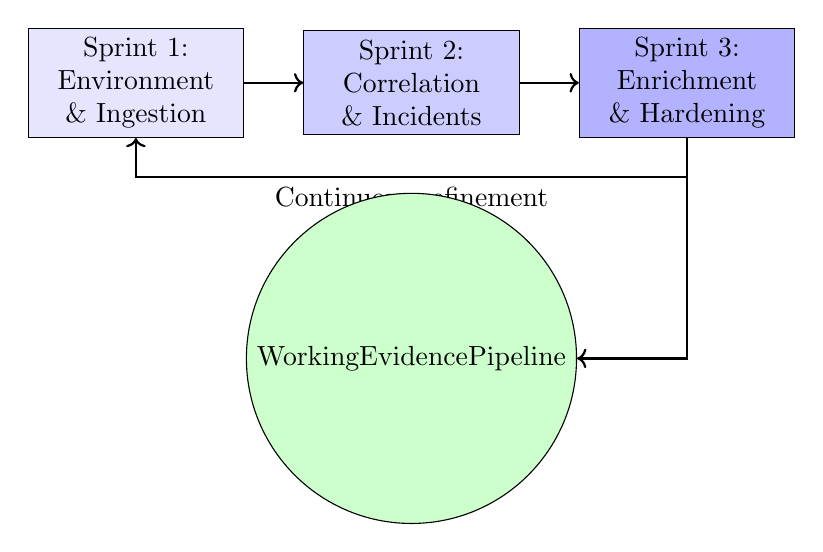
\begin{tikzpicture}[node distance=2cm, auto]
        \node[draw, rectangle, fill=blue!10, text width=2.5cm, align=center] (sprint1) {Sprint 1:\\Environment \& Ingestion};
        \node[draw, rectangle, fill=blue!20, text width=2.5cm, align=center, right of=sprint1, xshift=1.5cm] (sprint2) {Sprint 2:\\Correlation \& Incidents};
        \node[draw, rectangle, fill=blue!30, text width=2.5cm, align=center, right of=sprint2, xshift=1.5cm] (sprint3) {Sprint 3:\\Enrichment \& Hardening};

        \draw[thick, ->] (sprint1) -- (sprint2);
        \draw[thick, ->] (sprint2) -- (sprint3);
        \draw[thick, ->] (sprint3.south) |- ++(0,-0.5) -| (sprint1.south) node[pos=0.25, below] {Continuous refinement};

        \node[draw, circle, fill=green!20, below of=sprint2, yshift=-1.5cm] (delivery) {Working\\Evidence\\Pipeline};
        \draw[thick, ->] (sprint3) |- (delivery);
    \end{tikzpicture}
    \begin{itemize}
        \item \textbf{Flexibility:} adapting to real DevStack/OpenStack constraints as they appear.
        \item \textbf{Iteration:} each sprint hardens reliability before the next layer is added.
    \end{itemize}
\end{frame}

\begin{frame}{Project Management --- Task Table}
    \slidepurpose{Detail the tasks, their duration and the exact type of temporal link}{Organization / planning}
    \textbf{The table below refines the plan with lags and PERT relations.}
    \centering
    \scriptsize
    \renewcommand{\arraystretch}{1.1}
    \begin{adjustbox}{max width=0.98\textwidth}
    \begin{tabular}{|c|p{5.6cm}|c|p{4.8cm}|}
        \hline
        \textbf{ID} & \textbf{Task Name} & \textbf{Duration} & \textbf{Predecessor(s) + link} \\ \hline
        \textbf{A} & Onboarding \& problem framing (OpenStack, journald) & 3 d & --- \\ \hline
        \textbf{B} & SOTA study: log-based RCA \& streaming ingestion & 4 d & A (0FD) \\ \hline
        \textbf{C} & SOTA study: graph correlation \& incident detection & 4 d & A (0FD) \\ \hline
        \textbf{D} & SOTA study: local LLM reasoning (CoT) \& explainability & 2 d & B (1DD), C (0FF) \\ \hline
        \textbf{E} & Environment setup (DevStack, Tailscale, MongoDB) & 5 d & A (0FD) \\ \hline
        \textbf{F} & Ingestion \& parsing pipeline (raw $\to$ parsed logs) & 6 d & B (0FD), E (0FD) \\ \hline
        \textbf{G} & Correlation engine (event\_edges design) & 7 d & C (0FD), E (0FD) \\ \hline
        \textbf{H} & Incident integration on live correlated graph & 5 d & F (0FD), G (0FD) \\ \hline
        \textbf{I} & Enrichment worker (evidence package) & 4 d & H (0FD) \\ \hline
        \textbf{J} & Provider framework scaffolding & 2 d & A (1DD) \\ \hline
        \textbf{K} & Reliability hardening \& unit tests & 10 d & I (0FD), J (0FD) \\ \hline
        \textbf{L} & Validation \& end-to-end testing & 3 d & K (0FD) \\ \hline
        \textbf{M} & Final report, demo \& presentation & 5 d & L (0FD), D (0FD) \\ \hline
    \end{tabular}
    \end{adjustbox}

    \vspace{0.15cm}
    \tiny
    \begin{block}{Notation}
        \textbf{Example:} \texttt{0FD} means \emph{Finish-to-Start, no lag}; \texttt{1DD} means \emph{Start-to-Start with a 1-day lag}.
        General notation: \textbf{[lag] + [link type]}.
    \end{block}
\end{frame}

\begin{frame}{Project Management --- Float Table}
    \slidepurpose{Quantify the flexibility of each task through free and total float}{Organization / planning}
    \centering
    \scriptsize
    \renewcommand{\arraystretch}{1.28}
    \setlength{\tabcolsep}{4.2pt}
    \begin{adjustbox}{max width=0.98\textwidth}
    \begin{tabular}{|c|*{13}{c|}}
        \hline
        \textbf{ID} & \textbf{A} & \textbf{B} & \textbf{C} & \textbf{D} & \textbf{E} & \textbf{F} & \textbf{G} & \textbf{H} & \textbf{I} & \textbf{J} & \textbf{K} & \textbf{L} & \textbf{M} \\ \hline
        \textbf{FF} & 0 & 1 & 0 & 30 & 0 & 1 & 0 & 0 & 0 & 21 & 0 & 0 & 0 \\ \hline
        \textbf{TF} & 0 & 2 & 1 & 30 & 0 & 1 & 0 & 0 & 0 & 21 & 0 & 0 & 0 \\ \hline
    \end{tabular}
    \end{adjustbox}

    \vspace{0.2cm}
    \tiny
    \textbf{FF} = free float; \textbf{TF} = total float. Critical tasks verify \textbf{FF = TF = 0}, while \textbf{D} and \textbf{J} carry most of the schedule's slack.
    \begin{alertblock}{Critical Path}
        \textbf{A $\rightarrow$ E $\rightarrow$ G $\rightarrow$ H $\rightarrow$ I $\rightarrow$ K $\rightarrow$ L $\rightarrow$ M}
        \hfill \textbf{Estimated total duration: 42 days ($\approx$ 6-week internship)}
    \end{alertblock}
\end{frame}

\begin{frame}{Methodology --- PERT Network Diagram}
    \slidepurpose{Visualize the PERT network with earliest/latest dates and the critical path}{Organization / planning}
    \tikzsolutionfigure{
    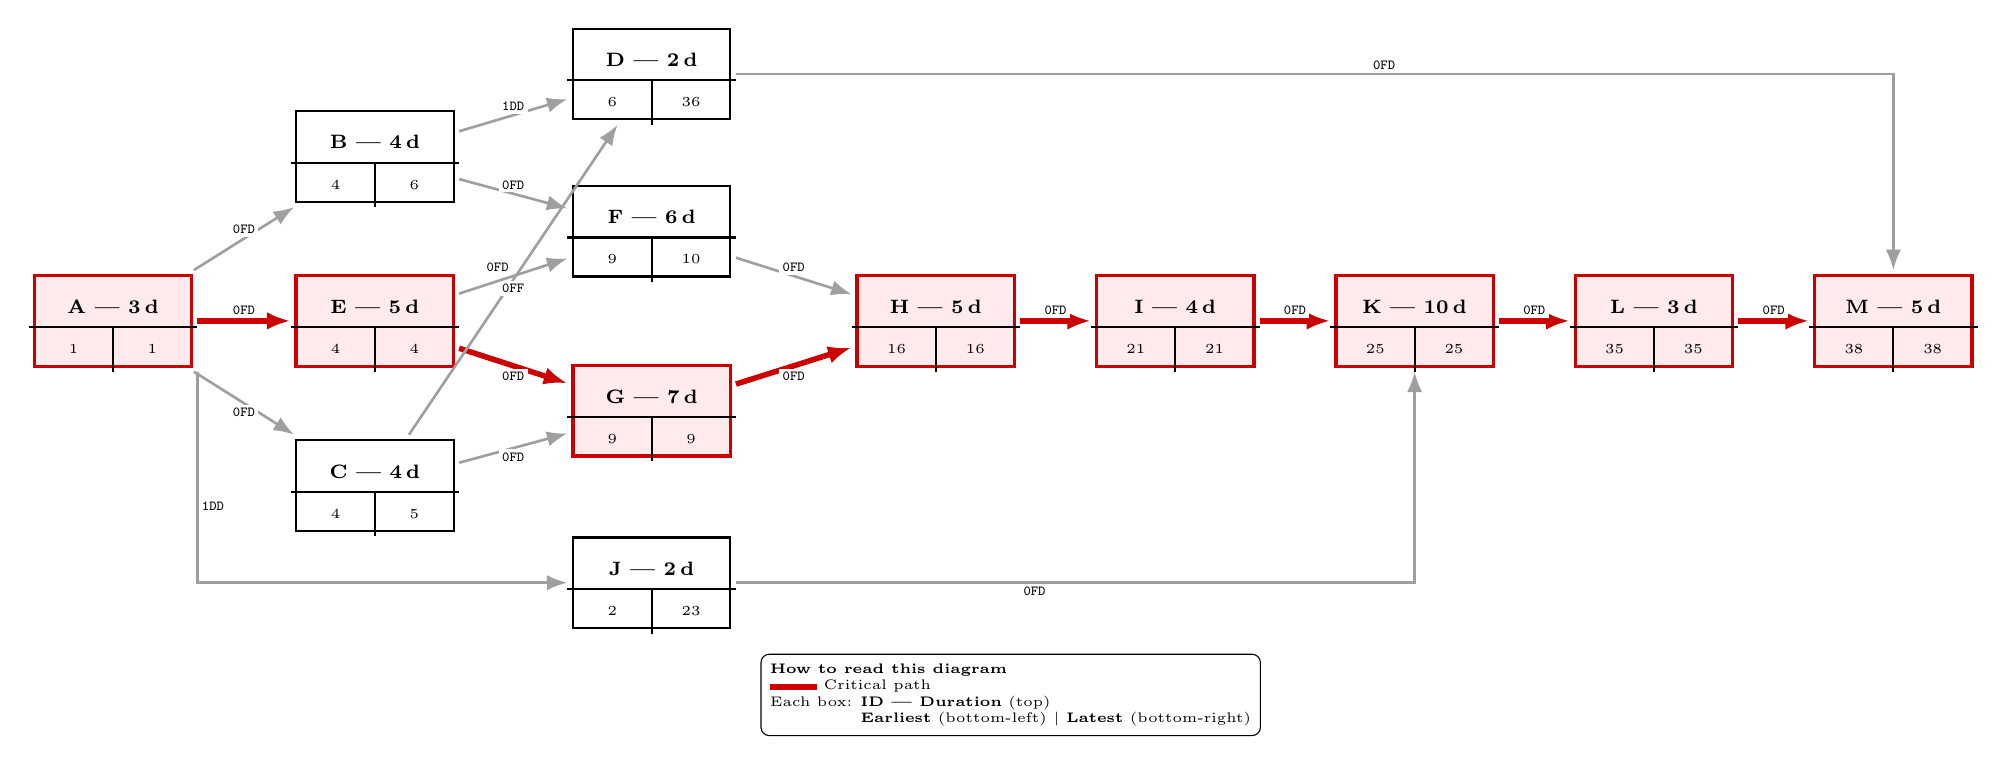
\begin{tikzpicture}[
        x=0.95cm,
        y=0.95cm,
        link/.style={-{Latex[length=2.6mm]}, line width=0.95pt, draw=gray!75},
        clink/.style={-{Latex[length=3mm]}, line width=2pt, draw=red!80!black},
        rel/.style={font=\tiny, fill=white, inner sep=1.2pt}
    ]
        \pertnode{A}{draw=red!80!black, very thick, fill=red!8}{(0,0)}{A --- 3\,d}{1}{1}
        \pertnode{B}{}{(3.5,2.2)}{B --- 4\,d}{4}{6}
        \pertnode{E}{draw=red!80!black, very thick, fill=red!8}{(3.5,0)}{E --- 5\,d}{4}{4}
        \pertnode{C}{}{(3.5,-2.2)}{C --- 4\,d}{4}{5}
        \pertnode{D}{}{(7.2,3.3)}{D --- 2\,d}{6}{36}
        \pertnode{F}{}{(7.2,1.2)}{F --- 6\,d}{9}{10}
        \pertnode{G}{draw=red!80!black, very thick, fill=red!8}{(7.2,-1.2)}{G --- 7\,d}{9}{9}
        \pertnode{J}{}{(7.2,-3.5)}{J --- 2\,d}{2}{23}
        \pertnode{H}{draw=red!80!black, very thick, fill=red!8}{(11,0)}{H --- 5\,d}{16}{16}
        \pertnode{I}{draw=red!80!black, very thick, fill=red!8}{(14.2,0)}{I --- 4\,d}{21}{21}
        \pertnode{K}{draw=red!80!black, very thick, fill=red!8}{(17.4,0)}{K --- 10\,d}{25}{25}
        \pertnode{L}{draw=red!80!black, very thick, fill=red!8}{(20.6,0)}{L --- 3\,d}{35}{35}
        \pertnode{M}{draw=red!80!black, very thick, fill=red!8}{(23.8,0)}{M --- 5\,d}{38}{38}

        \draw[clink] (A) -- node[rel, above] {\texttt{0FD}} (E);
        \draw[clink] (E) -- node[rel, below] {\texttt{0FD}} (G);
        \draw[clink] (G) -- node[rel, below] {\texttt{0FD}} (H);
        \draw[clink] (H) -- node[rel, above] {\texttt{0FD}} (I);
        \draw[clink] (I) -- node[rel, above] {\texttt{0FD}} (K);
        \draw[clink] (K) -- node[rel, above] {\texttt{0FD}} (L);
        \draw[clink] (L) -- node[rel, above] {\texttt{0FD}} (M);

        \draw[link] (A) -- node[rel, above] {\texttt{0FD}} (B);
        \draw[link] (A) -- node[rel, below] {\texttt{0FD}} (C);
        \draw[link] (A.south east) |- node[rel, pos=0.32, right] {\texttt{1DD}} (J.west);
        \draw[link] (B) -- node[rel, above] {\texttt{1DD}} (D);
        \draw[link] (C) -- node[rel, below] {\texttt{0FF}} (D);
        \draw[link] (B) -- node[rel, above] {\texttt{0FD}} (F);
        \draw[link] (E) -- node[rel, above left] {\texttt{0FD}} (F);
        \draw[link] (C) -- node[rel, below] {\texttt{0FD}} (G);
        \draw[link] (F) -- node[rel, above] {\texttt{0FD}} (H);
        \draw[link] (J.east) -| node[rel, pos=0.22, below] {\texttt{0FD}} (K.south);
        \draw[link] (D.east) -| node[rel, pos=0.28, above] {\texttt{0FD}} (M.north);

        \node[draw, rounded corners=3pt, fill=white, align=left, font=\tiny] at (12,-5) {
            \textbf{How to read this diagram}\\
            \textcolor{red!80!black}{\rule{0.6cm}{2pt}} Critical path\\
            Each box: \textbf{ID --- Duration} (top)\\
            \phantom{Each box: }\textbf{Earliest} (bottom-left) \textbar{} \textbf{Latest} (bottom-right)
        };
    \end{tikzpicture}
    }{PERT network of the OpenStack RCA Copilot with critical path and earliest/latest dates.}
\end{frame}

\begin{frame}{Project Management --- Gantt Chart}
    \slidepurpose{Project the schedule onto a 6-week internship calendar respecting the DD, FD and FF links}{Organization / planning}
    \centering
    \small
    \begin{adjustbox}{max width=0.98\textwidth, max totalheight=0.8\textheight}
    \begin{ganttchart}[
        hgrid,
        vgrid,
        x unit=0.222cm,
        y unit chart=0.50cm,
        y unit title=0.45cm,
        title height=1,
        bar height=0.66,
        group height=0.74,
        group peaks tip position=0,
        bar label font=\scriptsize,
        group label font=\scriptsize\bfseries,
        title label font=\scriptsize\bfseries,
        bar label node/.append style={align=left, text width=2.6cm},
        group label node/.append style={align=left},
        bar/.append style={fill=blue!18, draw=blue!70!black},
        group/.append style={fill=black!10, draw=black!65},
        link/.style={-Latex, line width=0.55pt, draw=black!60},
        link label font=\tiny
    ]{1}{42}
        \gantttitle{Internship Calendar (6 Weeks)}{42} \\
        \gantttitle{W1}{7}\gantttitle{W2}{7}\gantttitle{W3}{7}\gantttitle{W4}{7}\gantttitle{W5}{7}\gantttitle{W6}{7} \\

        \ganttgroup{Framing \& Analysis}{1}{8} \\
        \ganttbar[name=A, bar/.append style={fill=red!20, draw=red!75!black}]{A Onboarding}{1}{3} \\
        \ganttbar[name=B]{B SOTA ingestion}{4}{7} \\
        \ganttbar[name=C]{C SOTA correlation}{4}{7} \\
        \ganttbar[name=D]{D SOTA LLM/CoT}{6}{7} \\
        \ganttbar[name=E, bar/.append style={fill=red!20, draw=red!75!black}]{E Environment setup}{4}{8} \\
        \ganttbar[name=J]{J Provider fwk}{2}{3} \\

        \ganttgroup{Pipeline Development}{9}{24} \\
        \ganttbar[name=F]{F Ingestion+parsing}{9}{14} \\
        \ganttbar[name=G, bar/.append style={fill=red!20, draw=red!75!black}]{G Correlation engine}{9}{15} \\
        \ganttbar[name=H, bar/.append style={fill=red!20, draw=red!75!black}]{H Incident integr.}{16}{20} \\
        \ganttbar[name=I, bar/.append style={fill=red!20, draw=red!75!black}]{I Enrichment}{21}{24} \\

        \ganttgroup{Hardening \& Closure}{25}{42} \\
        \ganttbar[name=K, bar/.append style={fill=red!20, draw=red!75!black}]{K Hardening/tests}{25}{34} \\
        \ganttbar[name=L, bar/.append style={fill=red!20, draw=red!75!black}]{L Validation}{35}{37} \\
        \ganttbar[name=M, bar/.append style={fill=red!20, draw=red!75!black}]{M Report/demo}{38}{42} \\

        \ganttlink[link type=f-s, link label=FD]{A}{B}
        \ganttlink[link type=f-s, link label=FD]{A}{C}
        \ganttlink[link type=f-s, link label=FD]{A}{E}
        \ganttlink[link type=s-s, link label=DD+1]{A}{J}
        \ganttlink[link type=s-s, link label=DD+1]{B}{D}
        \ganttlink[link type=f-f, link label=FF]{C}{D}
        \ganttlink[link type=f-s, link label=FD]{B}{F}
        \ganttlink[link type=f-s, link label=FD]{E}{F}
        \ganttlink[link type=f-s, link label=FD]{C}{G}
        \ganttlink[link type=f-s, link label=FD]{E}{G}
        \ganttlink[link type=f-s, link label=FD]{F}{H}
        \ganttlink[link type=f-s, link label=FD]{G}{H}
        \ganttlink[link type=f-s, link label=FD]{H}{I}
        \ganttlink[link type=f-s, link label=FD]{I}{K}
        \ganttlink[link type=f-s, link label=FD]{J}{K}
        \ganttlink[link type=f-s, link label=FD]{K}{L}
        \ganttlink[link type=f-s, link label=FD]{L}{M}
        \ganttlink[link type=f-s, link label=FD]{D}{M}
    \end{ganttchart}
\end{adjustbox}

\end{frame}

\section{OpenStack and the Debugging Challenge}

\begin{frame}{OpenStack: A Powerful, Modular Cloud Platform}
\slidepurpose{Introduce the platform this project operates on}{Technical context}
\centering
\begin{adjustbox}{max width=0.94\linewidth, max height=0.40\textheight}
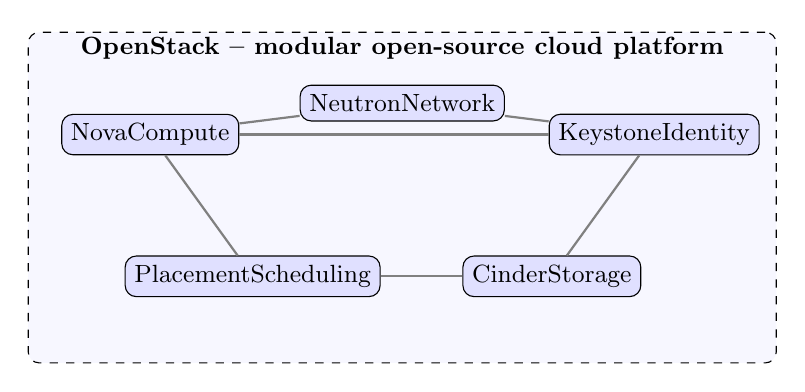
\begin{tikzpicture}[x=1cm,y=1cm, every node/.style={font=\small}]
    \node[draw, rounded corners, dashed, minimum width=9.5cm, minimum height=4.2cm, fill=blue!3] at (4.5,2) {};
    \node[font=\bfseries\small] at (4.5,3.9) {OpenStack -- modular open-source cloud platform};
    \node[draw, rectangle, rounded corners, fill=blue!12, minimum width=2cm] (nova) at (1.3,2.8) {Nova\\Compute};
    \node[draw, rectangle, rounded corners, fill=blue!12, minimum width=2cm] (neutron) at (4.5,3.2) {Neutron\\Network};
    \node[draw, rectangle, rounded corners, fill=blue!12, minimum width=2cm] (keystone) at (7.7,2.8) {Keystone\\Identity};
    \node[draw, rectangle, rounded corners, fill=blue!12, minimum width=2cm] (placement) at (2.6,1.0) {Placement\\Scheduling};
    \node[draw, rectangle, rounded corners, fill=blue!12, minimum width=2cm] (cinder) at (6.4,1.0) {Cinder\\Storage};
    \draw[thick, gray] (nova) -- (neutron);
    \draw[thick, gray] (neutron) -- (keystone);
    \draw[thick, gray] (nova) -- (placement);
    \draw[thick, gray] (keystone) -- (cinder);
    \draw[thick, gray] (placement) -- (cinder);
    \draw[thick, gray] (nova) -- (keystone);
\end{tikzpicture}
\end{adjustbox}
\vspace{0.15cm}
{\footnotesize
\begin{itemize}
    \item Leading open-source IaaS platform, deployed at large scale worldwide.
    \item Modular by design: independent services for compute, network, identity, storage.
    \item Powers Huawei Cloud Stack's own private / sovereign cloud offering.
\end{itemize}}
\end{frame}

\begin{frame}{The Cost of Modularity: Hard-to-Backtrace Failures}
\slidepurpose{Motivate why root-cause analysis needs automated assistance}{Technical context}
\centering
\begin{adjustbox}{max width=0.94\linewidth, max height=0.42\textheight}
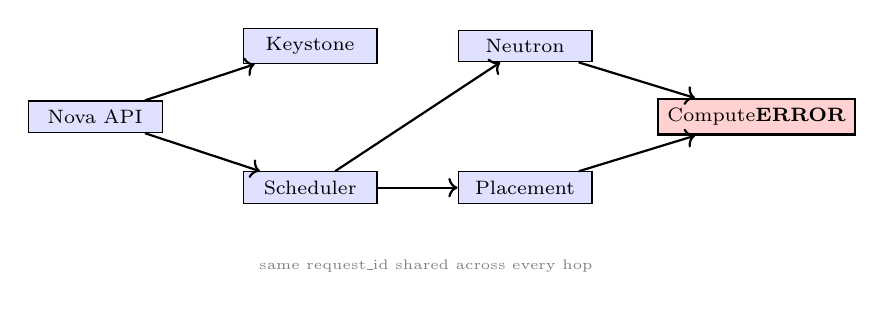
\begin{tikzpicture}[x=1.05cm,y=1cm, every node/.style={font=\scriptsize}]
    \node[draw, rectangle, fill=blue!12, minimum width=1.7cm] (api) at (0,2) {Nova API};
    \node[draw, rectangle, fill=blue!12, minimum width=1.7cm] (key) at (2.6,2.9) {Keystone};
    \node[draw, rectangle, fill=blue!12, minimum width=1.7cm] (sch) at (2.6,1.1) {Scheduler};
    \node[draw, rectangle, fill=blue!12, minimum width=1.7cm] (plac) at (5.2,1.1) {Placement};
    \node[draw, rectangle, fill=blue!12, minimum width=1.7cm] (neu) at (5.2,2.9) {Neutron};
    \node[draw, rectangle, fill=red!18, minimum width=1.9cm, thick] (comp) at (8,2) {Compute\\\textbf{ERROR}};
    \draw[->,thick] (api) -- (key);
    \draw[->,thick] (api) -- (sch);
    \draw[->,thick] (sch) -- (plac);
    \draw[->,thick] (sch) -- (neu);
    \draw[->,thick] (plac) -- (comp);
    \draw[->,thick] (neu) -- (comp);
    \node[font=\tiny, gray] at (4,0.1) {same request\_id shared across every hop};
\end{tikzpicture}
\end{adjustbox}
\vspace{0.15cm}
{\footnotesize
\begin{itemize}
    \item Every strength above is also a debugging liability: one failure, many possible origins.
    \item A Nova error can trace back to Neutron, Keystone, Placement, or a stale event minutes earlier.
    \item Manually retracing this by hand does not scale -- this is exactly where AI assistance earns its place.
\end{itemize}}
\end{frame}

\section{Data Ingestion and Structuring Pipeline}

\begin{frame}{Step 1: Why Logs Go to journald}
\slidepurpose{Explain why logs are centralized through journald}{Pipeline -- ingestion}
\centering
\begin{adjustbox}{max width=0.94\linewidth, max height=0.40\textheight}
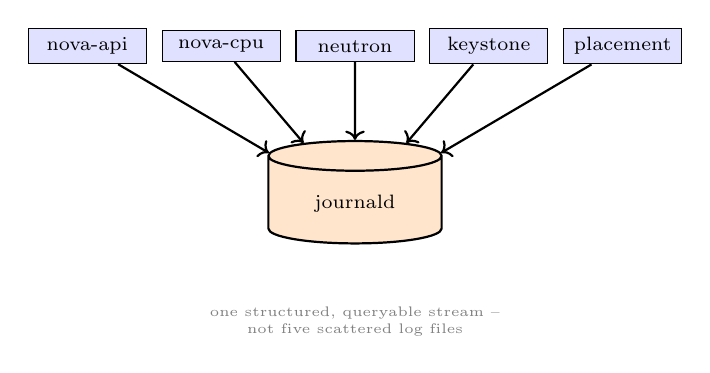
\begin{tikzpicture}[x=1cm,y=1cm, every node/.style={font=\scriptsize}]
    \node[draw, rectangle, fill=blue!12, minimum width=1.5cm] (napi) at (0.3,2.6) {nova-api};
    \node[draw, rectangle, fill=blue!12, minimum width=1.5cm] (ncpu) at (2.0,2.6) {nova-cpu};
    \node[draw, rectangle, fill=blue!12, minimum width=1.5cm] (neu) at (3.7,2.6) {neutron};
    \node[draw, rectangle, fill=blue!12, minimum width=1.5cm] (key) at (5.4,2.6) {keystone};
    \node[draw, rectangle, fill=blue!12, minimum width=1.5cm] (plc) at (7.1,2.6) {placement};
    \node[draw, cylinder, shape border rotate=90, aspect=0.3, fill=orange!20, minimum width=2.2cm, minimum height=1.3cm, thick] (j) at (3.7,0.6) {journald};
    \draw[->, thick] (napi) -- (j);
    \draw[->, thick] (ncpu) -- (j);
    \draw[->, thick] (neu) -- (j);
    \draw[->, thick] (key) -- (j);
    \draw[->, thick] (plc) -- (j);
    \node[font=\tiny, gray, align=center] at (3.7,-0.9) {one structured, queryable stream --\\not five scattered log files};
\end{tikzpicture}
\end{adjustbox}
\vspace{0.15cm}
{\footnotesize
\begin{itemize}
    \item DevStack runs every OpenStack service as a systemd unit.
    \item journald gives ONE structured, queryable interface for all of them.
    \item No more hunting through separate files under /var/log/nova, /var/log/neutron...
\end{itemize}}
\end{frame}

\begin{frame}{Ingestion Is a Streaming Problem}
\slidepurpose{Explain why ingestion is a live streaming problem, not a batch read}{Pipeline -- ingestion}
\centering
\begin{adjustbox}{max width=0.94\linewidth, max height=0.40\textheight}
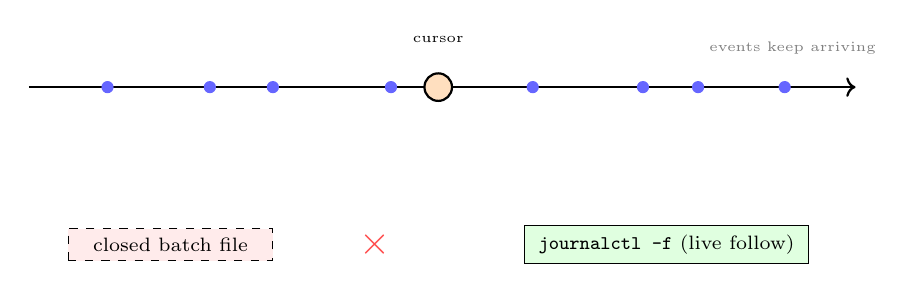
\begin{tikzpicture}[x=1cm,y=1cm, every node/.style={font=\scriptsize}]
    \draw[thick, ->] (0,1.5) -- (10.5,1.5);
    \foreach \x in {1,2.3,3.1,4.6,5.2,6.4,7.8,8.5,9.6}{
        \fill[blue!60] (\x,1.5) circle (2.2pt);
    }
    \node[draw, fill=orange!25, circle, thick, minimum size=0.35cm] (cursor) at (5.2,1.5) {};
    \node[font=\tiny] at (5.2,2.1) {cursor};
    \node[font=\tiny, gray] at (9.7,2.0) {events keep arriving};
    \node[draw, rectangle, fill=red!8, dashed, minimum width=2.6cm] at (1.8,-0.5) {closed batch file};
    \node[font=\Large, red!70] at (4.4,-0.5) {$\times$};
    \node[draw, rectangle, fill=green!12, minimum width=3.6cm] at (8.1,-0.5) {\texttt{journalctl -f} (live follow)};
\end{tikzpicture}
\end{adjustbox}
\vspace{0.15cm}
{\footnotesize
\begin{itemize}
    \item Logs never stop while OpenStack runs -- there is no ``finished file'' to read once.
    \item The collector follows the journal live, the same way you would \texttt{tail -f}.
    \item Every read is resumable via a cursor, or a crash loses the ``where was I.''
\end{itemize}}
\end{frame}

\begin{frame}{From journald to MongoDB (raw\_logs)}
\slidepurpose{Show how logs travel from journald to durable storage}{Pipeline -- ingestion}
\centering
\begin{adjustbox}{max width=0.94\linewidth, max height=0.40\textheight}
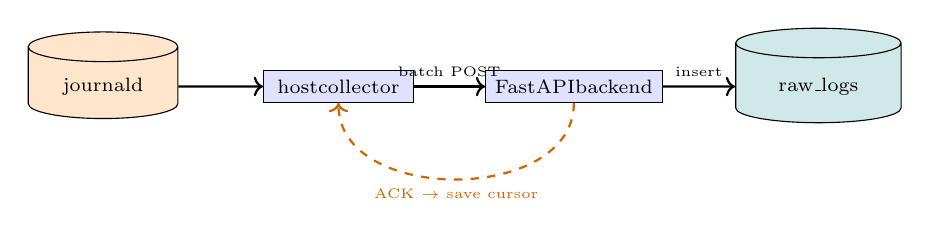
\begin{tikzpicture}[x=1.15cm,y=1cm, every node/.style={font=\scriptsize}]
    \node[draw, cylinder, shape border rotate=90, aspect=0.3, fill=orange!20, minimum width=1.9cm, minimum height=1.1cm] (j) at (0,1.7) {journald};
    \node[draw, rectangle, fill=blue!12, minimum width=1.9cm] (col) at (2.6,1.7) {host\\collector};
    \node[draw, rectangle, fill=blue!12, minimum width=1.9cm] (api) at (5.2,1.7) {FastAPI\\backend};
    \node[draw, cylinder, shape border rotate=90, aspect=0.3, fill=teal!18, minimum width=2.1cm, minimum height=1.2cm] (raw) at (7.9,1.7) {raw\_logs};
    \draw[->, thick] (j) -- (col);
    \draw[->, thick] (col) -- node[above,font=\tiny]{batch POST} (api);
    \draw[->, thick] (api) -- node[above,font=\tiny]{insert} (raw);
    \draw[->, thick, dashed, orange!80!black] (api.south) .. controls (5.2,0.2) and (2.6,0.2) .. (col.south) node[midway,below,font=\tiny]{ACK $\to$ save cursor};
\end{tikzpicture}
\end{adjustbox}
\vspace{0.15cm}
{\footnotesize
\begin{itemize}
    \item Batches of about 50 records (or every 2 s) are POSTed to the backend.
    \item The cursor is saved only \emph{after} a successful ACK -- crash-safe delivery.
    \item Duplicates are caught by a (boot\_id + journal\_cursor) unique index.
\end{itemize}}
\end{frame}

\begin{frame}{Step 2: From Raw Text to Structured Events}
\slidepurpose{Show how raw text becomes structured, queryable events}{Pipeline -- structuring}
\centering
\begin{adjustbox}{max width=0.94\linewidth, max height=0.40\textheight}
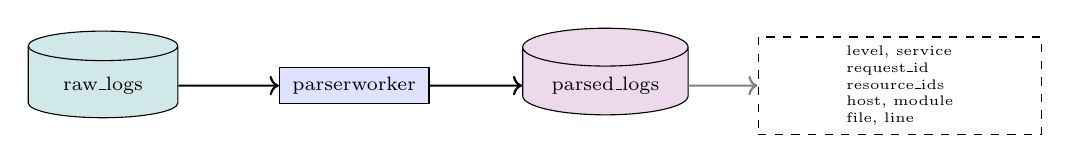
\begin{tikzpicture}[x=1.1cm,y=1cm, every node/.style={font=\scriptsize}]
    \node[draw, cylinder, shape border rotate=90, aspect=0.3, fill=teal!18, minimum width=1.9cm, minimum height=1.1cm] (raw) at (0,1.5) {raw\_logs};
    \node[draw, rectangle, fill=blue!12, minimum width=1.9cm] (parser) at (2.9,1.5) {parser\\worker};
    \node[draw, cylinder, shape border rotate=90, aspect=0.3, fill=violet!15, minimum width=2.1cm, minimum height=1.1cm] (parsed) at (5.8,1.5) {parsed\_logs};
    \node[draw, rectangle, dashed, fill=white, align=left, font=\tiny, minimum width=3.6cm] (fields) at (9.2,1.5) {level, service\\request\_id\\resource\_ids\\host, module\\file, line};
    \draw[->, thick] (raw) -- (parser);
    \draw[->, thick] (parser) -- (parsed);
    \draw[->, thick, gray] (parsed) -- (fields);
\end{tikzpicture}
\end{adjustbox}
\vspace{0.15cm}
{\footnotesize
\begin{itemize}
    \item A separate parser worker reads raw\_logs and writes parsed\_logs -- decoupled from ingestion.
    \item Extracts level, service, request\_id, resource\_ids, host, module, file, line.
    \item Parse failures are stored too (\texttt{parse\_status="failure"}), never silently dropped.
\end{itemize}}
\end{frame}

\begin{frame}{Project Structure: Why This Layout}
\slidepurpose{Justify the repository layout and link to the source}{Pipeline -- structuring}
\centering
\begin{adjustbox}{max width=0.96\linewidth, max height=0.42\textheight}
\begin{tikzpicture}[x=1cm,y=1cm, every node/.style={font=\scriptsize}]
    \node[draw, rectangle, fill=blue!12, minimum width=1.7cm] (col) at (0.3,2.6) {collector/};
    \node[draw, rectangle, fill=blue!12, minimum width=1.6cm] (be) at (2.5,2.6) {backend/};
    \node[draw, rectangle, fill=violet!15, minimum width=2.3cm] (par) at (5.0,2.6) {parser\_worker/};
    \node[draw, rectangle, fill=violet!15, minimum width=2.7cm] (corr) at (7.9,2.6) {correlation\_worker/};
    \node[draw, rectangle, fill=orange!15, minimum width=2.3cm] (inc) at (3.4,0.8) {incident\_worker/};
    \node[draw, rectangle, fill=orange!15, minimum width=2.7cm] (enr) at (6.4,0.8) {enrichment\_worker/};
    \draw[->, thick] (col) -- (be);
    \draw[->, thick] (be) -- (par);
    \draw[->, thick] (par) -- (corr);
    \draw[->, thick] (corr.south) |- (inc.east);
    \draw[->, thick] (inc) -- (enr);
    \node[anchor=west] (qr) at (9.6,2.3) {
\includegraphics[width=2.0cm]{qrcode_ghub.png}};
    \node[font=\tiny, gray, anchor=west, align=left] at (9.55,0.7) {carteeeltheboss/\\RCA\_copilot -- MIT};
\end{tikzpicture}
\end{adjustbox}
\vspace{0.15cm}
{\footnotesize
\begin{itemize}
    \item One folder per pipeline stage: independently testable, independently deployable.
    \item Python + Docker Compose + pytest -- MIT-licensed, open source.
    \item Full source and docs -- scan the QR code to open the repository.
\end{itemize}}
\end{frame}

\section{Correlation Graph and Evidence Package}

\begin{frame}{Why This Is a Graph Problem}
\slidepurpose{Justify why correlation is modeled as a graph, not a table}{Correlation -- design}
\centering
\begin{adjustbox}{max width=0.94\linewidth, max height=0.42\textheight}
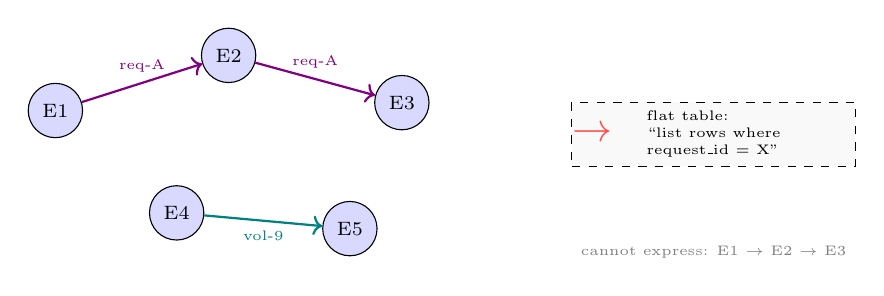
\begin{tikzpicture}[x=1.1cm,y=1cm, every node/.style={font=\scriptsize}]
    \node[draw, circle, fill=blue!15] (a) at (0,2.4) {E1};
    \node[draw, circle, fill=blue!15] (b) at (2,3.1) {E2};
    \node[draw, circle, fill=blue!15] (c) at (4,2.5) {E3};
    \node[draw, circle, fill=blue!15] (d) at (1.4,1.1) {E4};
    \node[draw, circle, fill=blue!15] (e) at (3.4,0.9) {E5};
    \draw[->, thick, violet] (a) -- node[above,font=\tiny]{req-A} (b);
    \draw[->, thick, violet] (b) -- node[above,font=\tiny]{req-A} (c);
    \draw[->, thick, teal] (d) -- node[below,font=\tiny]{vol-9} (e);
    \node[draw, rectangle, dashed, fill=gray!5, align=left, font=\tiny, minimum width=3.6cm] at (7.6,2.1) {flat table:\\``list rows where\\request\_id = X''};
    \node[font=\Large, red!70] at (6.2,2.1) {$\to$};
    \node[font=\tiny, gray] at (7.6,0.6) {cannot express: E1 $\to$ E2 $\to$ E3};
\end{tikzpicture}
\end{adjustbox}
\vspace{0.15cm}
{\footnotesize
\begin{itemize}
    \item Root-cause investigation asks ``what led to what'' -- a chain question, not a filter question.
    \item Shared request\_id / resource\_id are natural EDGES between event NODES.
    \item A flat table can list matches; only a graph expresses a multi-hop evidence chain.
\end{itemize}}
\end{frame}

\begin{frame}{Building Correlation Edges Correctly}
\slidepurpose{Define the two deterministic correlation rules}{Correlation -- design}
\centering
\begin{adjustbox}{max width=0.94\linewidth, max height=0.42\textheight}
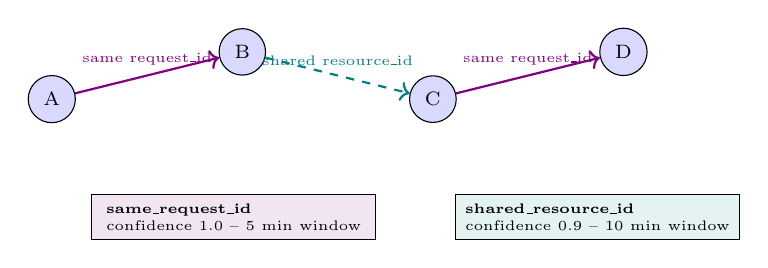
\begin{tikzpicture}[x=1.1cm,y=1cm, every node/.style={font=\scriptsize}]
    \node[draw, circle, fill=blue!15] (a) at (0,1.6) {A};
    \node[draw, circle, fill=blue!15] (b) at (2.2,2.2) {B};
    \node[draw, circle, fill=blue!15] (c) at (4.4,1.6) {C};
    \node[draw, circle, fill=blue!15] (d) at (6.6,2.2) {D};
    \draw[->, thick, violet] (a) -- node[above,font=\tiny]{same request\_id} (b);
    \draw[->, thick, teal, dashed] (b) -- node[above,font=\tiny]{shared resource\_id} (c);
    \draw[->, thick, violet] (c) -- node[above,font=\tiny]{same request\_id} (d);
    \node[draw, rectangle, fill=violet!10, font=\tiny, align=left, minimum width=3.6cm] at (2.1,0.1) {\textbf{same\_request\_id}\\confidence 1.0 -- 5 min window};
    \node[draw, rectangle, fill=teal!10, font=\tiny, align=left, minimum width=3.6cm] at (6.3,0.1) {\textbf{shared\_resource\_id}\\confidence 0.9 -- 10 min window};
\end{tikzpicture}
\end{adjustbox}
\vspace{0.15cm}
{\footnotesize
\begin{itemize}
    \item Two deterministic rules only -- no black-box guessing.
    \item Every edge carries a reason and a confidence score.
    \item Edges are directed and chronological (earlier $\to$ later) -- correlation, never proof of cause.
\end{itemize}}
\end{frame}

\begin{frame}{Avoiding the $O(n^2)$ Explosion}
\slidepurpose{Show the engineering fix that keeps the graph readable}{Correlation -- design}
\centering
\begin{adjustbox}{max width=0.94\linewidth, max height=0.42\textheight}
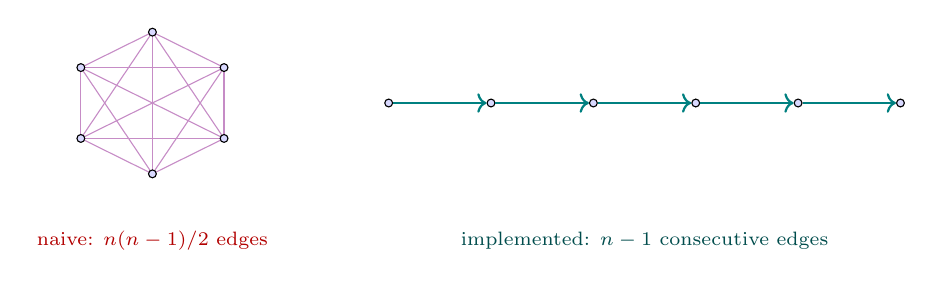
\begin{tikzpicture}[x=1cm,y=1cm, every node/.style={font=\tiny}]
    \foreach \i/\ang in {1/90,2/30,3/-30,4/-90,5/-150,6/150}{
        \coordinate (p\i) at ({1.6+1.05*cos(\ang)},{1.9+0.9*sin(\ang)});
    }
    \begin{scope}[on background layer]
        \foreach \i in {1,...,5}{
            \pgfmathtruncatemacro{\s}{\i+1}
            \foreach \j in {\s,...,6}{\draw[violet!45, thin] (p\i) -- (p\j);}
        }
    \end{scope}
    \foreach \i in {1,...,6}{\node[draw,circle,fill=blue!15,inner sep=1pt] at (p\i) {};}
    \node[font=\scriptsize, red!70!black] at (1.6,0.15) {naive: $n(n-1)/2$ edges};
    \foreach \i/\x in {1/4.6,2/5.9,3/7.2,4/8.5,5/9.8,6/11.1}{\node[draw,circle,fill=blue!15,inner sep=1pt] (c\i) at (\x,1.9) {};}
    \foreach \i/\j in {1/2,2/3,3/4,4/5,5/6}{\draw[->, thick, teal] (c\i) -- (c\j);}
    \node[font=\scriptsize, teal!60!black] at (7.85,0.15) {implemented: $n-1$ consecutive edges};
\end{tikzpicture}
\end{adjustbox}
\vspace{0.15cm}
{\footnotesize
\begin{itemize}
    \item Naively linking every pair inside a shared-ID group explodes combinatorially.
    \item Fix: sort by time, link consecutive events only -- skip periodic/noisy groups entirely.
    \item Same coverage, a fraction of the edges -- a graph a human can actually read.
\end{itemize}}
\end{frame}

\begin{frame}{From Seed Event to Bounded Incident}
\slidepurpose{Show how a seed event becomes a bounded incident}{Correlation -- incidents}
\centering
\begin{adjustbox}{max width=0.94\linewidth, max height=0.42\textheight}
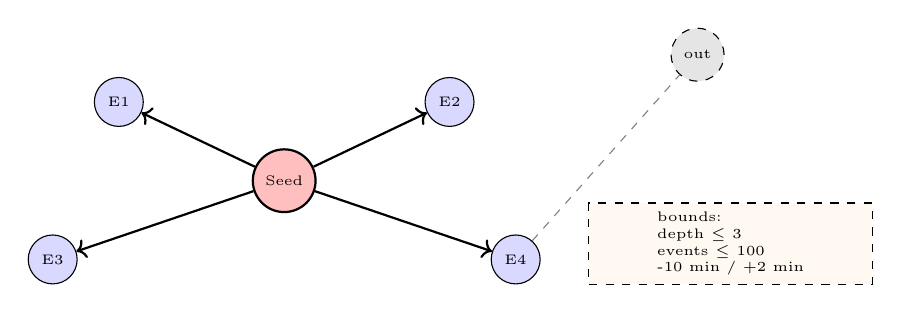
\begin{tikzpicture}[x=1.05cm,y=1cm, every node/.style={font=\tiny}]
    \node[draw, circle, fill=red!25, thick] (s) at (4,1.8) {Seed};
    \node[draw, circle, fill=blue!15] (a) at (2,2.8) {E1};
    \node[draw, circle, fill=blue!15] (b) at (6,2.8) {E2};
    \node[draw, circle, fill=blue!15] (c) at (1.2,0.8) {E3};
    \node[draw, circle, fill=blue!15] (d) at (6.8,0.8) {E4};
    \node[draw, circle, fill=gray!20, dashed] (out) at (9,3.4) {out};
    \draw[->, thick] (s) -- (a);
    \draw[->, thick] (s) -- (b);
    \draw[->, thick] (s) -- (c);
    \draw[->, thick] (s) -- (d);
    \draw[gray, dashed] (d) -- (out);
    \node[draw, rectangle, dashed, fill=orange!5, align=left, font=\tiny, minimum width=3.6cm] at (9.4,1) {bounds:\\depth $\le$ 3\\events $\le$ 100\\-10 min / +2 min};
\end{tikzpicture}
\end{adjustbox}
\vspace{0.15cm}
{\footnotesize
\begin{itemize}
    \item Seed rules: ERROR/CRITICAL, Traceback, Exception, failed/timeout, resource ERROR state.
    \item Obvious false positives (e.g. ``0 failures'') are suppressed automatically.
    \item Bounded traversal keeps every incident small, readable, and explainable.
\end{itemize}}
\end{frame}

\begin{frame}{The Deterministic Evidence Package}
\slidepurpose{Show the deterministic package the AI layer will consume}{Correlation -- evidence}
\centering
\begin{adjustbox}{max width=0.94\linewidth, max height=0.40\textheight}
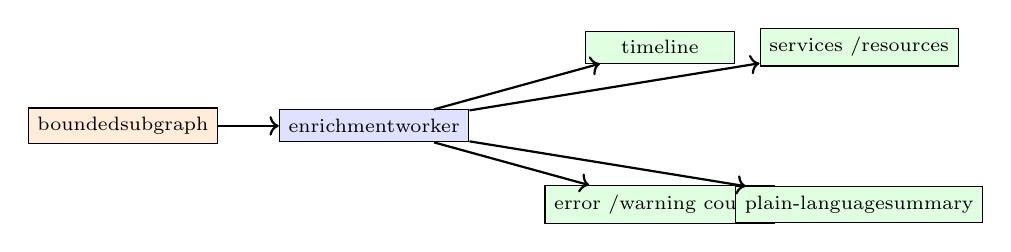
\begin{tikzpicture}[x=1.1cm,y=1cm, every node/.style={font=\scriptsize}]
    \node[draw, rectangle, fill=orange!15, minimum width=2.3cm] (sub) at (0,1.6) {bounded\\subgraph};
    \node[draw, rectangle, fill=blue!12, minimum width=2.3cm] (en) at (2.9,1.6) {enrichment\\worker};
    \node[draw, rectangle, fill=green!12, minimum width=1.9cm] (t1) at (6.2,2.6) {timeline};
    \node[draw, rectangle, fill=green!12, minimum width=1.9cm] (t2) at (8.5,2.6) {services /\\resources};
    \node[draw, rectangle, fill=green!12, minimum width=1.9cm] (t3) at (6.2,0.6) {error /\\warning counts};
    \node[draw, rectangle, fill=green!12, minimum width=1.9cm] (t4) at (8.5,0.6) {plain-language\\summary};
    \draw[->, thick] (sub) -- (en);
    \draw[->, thick] (en) -- (t1);
    \draw[->, thick] (en) -- (t2);
    \draw[->, thick] (en) -- (t3);
    \draw[->, thick] (en) -- (t4);
\end{tikzpicture}
\end{adjustbox}
\vspace{0.15cm}
{\footnotesize
\begin{itemize}
    \item Built entirely from stored events and edges -- zero AI involved at this stage.
    \item Ordered timeline, impacted services/resources, error/warning counts, summary.
    \item This package -- not raw logs -- is what the LLM will eventually reason over.
\end{itemize}}
\end{frame}

\section{AI Reasoning Layer}

\begin{frame}{Why Root-Cause Reasoning Needs Chain-of-Thought}
\slidepurpose{Explain why root-cause reasoning benefits from Chain-of-Thought}{AI layer -- reasoning}
\centering
\begin{adjustbox}{max width=0.94\linewidth, max height=0.42\textheight}
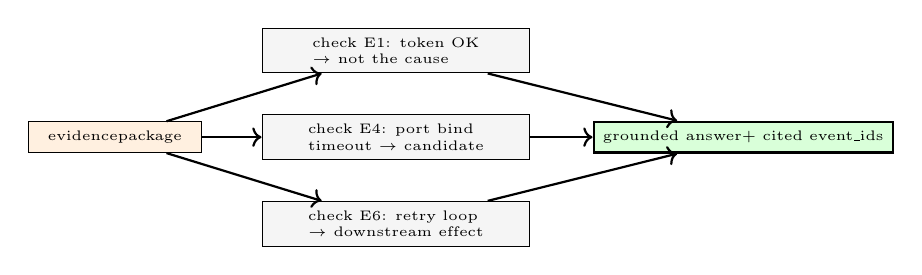
\begin{tikzpicture}[x=1.05cm,y=1cm, every node/.style={font=\tiny}]
    \node[draw, rectangle, fill=orange!12, minimum width=2.2cm] (ev) at (0,1.6) {evidence\\package};
    \node[draw, rectangle, fill=gray!8, align=left, minimum width=3.4cm] (h1) at (3.4,2.7) {check E1: token OK\\$\to$ not the cause};
    \node[draw, rectangle, fill=gray!8, align=left, minimum width=3.4cm] (h2) at (3.4,1.6) {check E4: port bind\\timeout $\to$ candidate};
    \node[draw, rectangle, fill=gray!8, align=left, minimum width=3.4cm] (h3) at (3.4,0.5) {check E6: retry loop\\$\to$ downstream effect};
    \node[draw, rectangle, thick, fill=green!15, minimum width=2.6cm] (ans) at (7.6,1.6) {grounded answer\\+ cited event\_ids};
    \draw[->, thick] (ev) -- (h1);
    \draw[->, thick] (ev) -- (h2);
    \draw[->, thick] (ev) -- (h3);
    \draw[->, thick] (h1) -- (ans);
    \draw[->, thick] (h2) -- (ans);
    \draw[->, thick] (h3) -- (ans);
\end{tikzpicture}
\end{adjustbox}
\vspace{0.15cm}
{\footnotesize
\begin{itemize}
    \item A single stacked failure often has several plausible explanations.
    \item Chain-of-Thought: the model checks hypotheses one by one, out loud, before concluding.
    \item Every claim must cite a real event\_id -- no free-floating guesses.
\end{itemize}}
\end{frame}

\begin{frame}{The Model: Ollama + DeepSeek-R1}
\slidepurpose{Introduce the local reasoning model used for explanation}{AI layer -- model choice}
\centering
\begin{adjustbox}{max width=0.94\linewidth, max height=0.40\textheight}
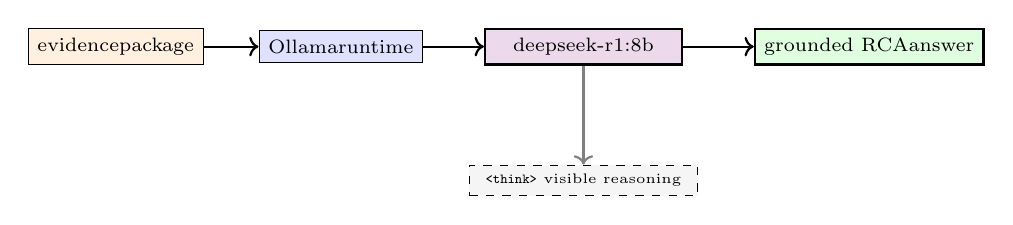
\begin{tikzpicture}[x=1.1cm,y=1cm, every node/.style={font=\scriptsize}]
    \node[draw, rectangle, fill=orange!12, minimum width=2.1cm] (ev) at (0,1.5) {evidence\\package};
    \node[draw, rectangle, fill=blue!12, minimum width=1.9cm] (ol) at (2.6,1.5) {Ollama\\runtime};
    \node[draw, rectangle, thick, fill=violet!15, minimum width=2.5cm] (ds) at (5.4,1.5) {deepseek-r1:8b};
    \node[draw, rectangle, dashed, fill=gray!8, minimum width=2.9cm, font=\tiny] (think) at (5.4,-0.2) {\texttt{<think>} visible reasoning};
    \node[draw, rectangle, thick, fill=green!12, minimum width=2.3cm] (ans) at (8.7,1.5) {grounded RCA\\answer};
    \draw[->, thick] (ev) -- (ol);
    \draw[->, thick] (ol) -- (ds);
    \draw[->, thick] (ds) -- (ans);
    \draw[->, thick, gray] (ds) -- (think);
\end{tikzpicture}
\end{adjustbox}
\vspace{0.15cm}
{\footnotesize
\begin{itemize}
    \item \texttt{deepseek-r1:8b}, served locally through Ollama -- MIT-licensed, open weights.
    \item Reasoning is visible (\texttt{<think>} tokens) -- transparent, auditable.
    \item A distilled reasoning model: near-frontier reasoning at laptop-GPU scale.
\end{itemize}}
\end{frame}

\begin{frame}{Prompt Engineering: Grounding the LLM in Evidence}
\slidepurpose{Show how the evidence package is turned into a grounded prompt}{AI layer -- prompting}
\centering
\begin{adjustbox}{max width=0.96\linewidth, max height=0.44\textheight}
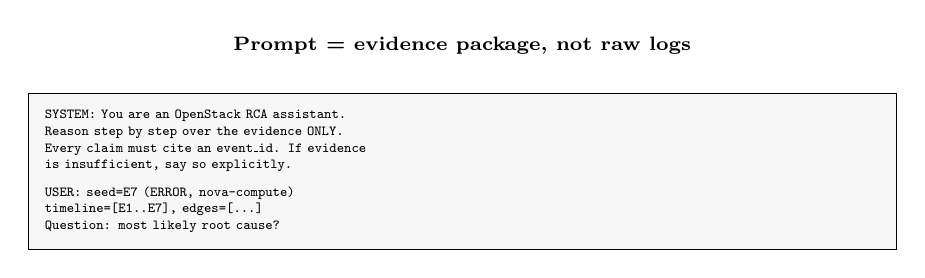
\begin{tikzpicture}[x=1cm,y=1cm]
    \node[draw, rectangle, fill=gray!6, align=left, font=\tiny\ttfamily, text width=10.6cm, inner sep=6pt] at (5.3,1.5) {
    SYSTEM: You are an OpenStack RCA assistant.\\
    Reason step by step over the evidence ONLY.\\
    Every claim must cite an event\_id. If evidence\\
    is insufficient, say so explicitly.\\[4pt]
    USER: seed=E7 (ERROR, nova-compute)\\
    timeline=[E1..E7], edges=[...]\\
    Question: most likely root cause?
    };
    \node[font=\bfseries\scriptsize] at (5.3,3.1) {Prompt = evidence package, not raw logs};
\end{tikzpicture}
\end{adjustbox}
\vspace{0.15cm}
{\footnotesize
\begin{itemize}
    \item The prompt IS the structured evidence package, not the raw logs.
    \item System prompt hard-requires a cited event\_id for every claim.
    \item Same contract works behind any future provider (Ollama today, others later).
\end{itemize}}
\end{frame}

\begin{frame}{Hardware: Two Machines, One Pipeline}
\slidepurpose{Describe the physical machines the pipeline runs on}{AI layer -- infrastructure}
\centering
\begin{adjustbox}{max width=0.94\linewidth, max height=0.42\textheight}
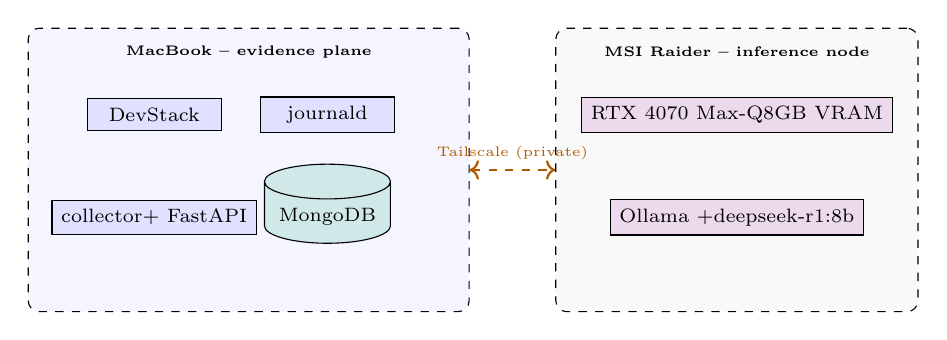
\begin{tikzpicture}[x=1cm,y=1cm, every node/.style={font=\scriptsize}]
    \node[draw, dashed, rounded corners, minimum width=5.6cm, minimum height=3.6cm, fill=blue!4] (mac) at (2.2,1.7) {};
    \node[font=\bfseries\tiny] at (2.2,3.2) {MacBook -- evidence plane};
    \node[draw, rectangle, fill=blue!12, minimum width=1.7cm] at (1.0,2.4) {DevStack};
    \node[draw, rectangle, fill=blue!12, minimum width=1.7cm] at (3.2,2.4) {journald};
    \node[draw, rectangle, fill=blue!12, minimum width=1.7cm] at (1.0,1.1) {collector\\+ FastAPI};
    \node[draw, cylinder, shape border rotate=90, aspect=0.3, fill=teal!18, minimum width=1.6cm, minimum height=1cm] at (3.2,1.1) {MongoDB};
    \node[draw, dashed, rounded corners, minimum width=4.6cm, minimum height=3.6cm, fill=gray!5] (msi) at (8.4,1.7) {};
    \node[font=\bfseries\tiny] at (8.4,3.2) {MSI Raider -- inference node};
    \node[draw, rectangle, fill=violet!15, minimum width=2.3cm] at (8.4,2.4) {RTX 4070 Max-Q\\8GB VRAM};
    \node[draw, rectangle, fill=violet!15, minimum width=2.3cm] at (8.4,1.1) {Ollama +\\deepseek-r1:8b};
    \draw[<->, thick, dashed, orange!70!black] (mac) -- node[above,font=\tiny]{Tailscale (private)} (msi);
\end{tikzpicture}
\end{adjustbox}
\vspace{0.15cm}
{\footnotesize
\begin{itemize}
    \item MacBook: DevStack, journald, collector, FastAPI, MongoDB -- the evidence plane.
    \item MSI Raider (RTX 4070 Max-Q, 8GB VRAM): local inference node.
    \item Linked privately over Tailscale -- no public exposure, no cloud hop.
\end{itemize}}
\end{frame}

\begin{frame}{Why DeepSeek-R1 Fits This Hardware}
\slidepurpose{Justify the model choice against the available VRAM}{AI layer -- infrastructure}
\centering
\begin{adjustbox}{max width=0.9\linewidth, max height=0.36\textheight}
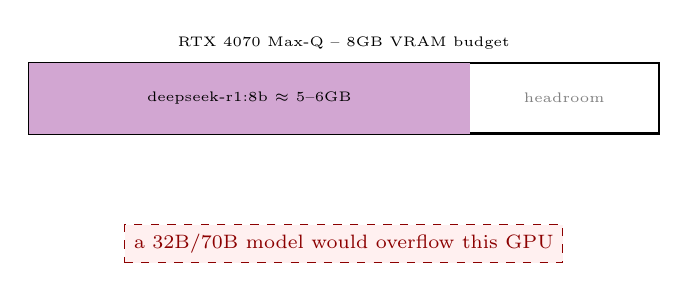
\begin{tikzpicture}[x=1cm,y=1cm, every node/.style={font=\scriptsize}]
    \draw[thick] (0,2) rectangle (8,2.9);
    \node[font=\tiny] at (4,3.15) {RTX 4070 Max-Q -- 8GB VRAM budget};
    \fill[violet!35] (0,2) rectangle (5.6,2.9);
    \node[font=\tiny] at (2.8,2.45) {deepseek-r1:8b $\approx$ 5--6GB};
    \node[font=\tiny, gray] at (6.8,2.45) {headroom};
    \node[draw, rectangle, dashed, red!55!black, fill=red!6, minimum width=4.6cm] at (4,0.6) {a 32B/70B model would overflow this GPU};
\end{tikzpicture}
\end{adjustbox}
\vspace{0.2cm}
{\footnotesize
\begin{itemize}
    \item Quantized \texttt{deepseek-r1:8b} fits comfortably inside 8GB of VRAM.
    \item Retains step-by-step reasoning distilled from the full R1 model.
    \item Right-sized: bigger models overflow this GPU, smaller ones reason worse.
\end{itemize}}
\end{frame}

\section{Data Sovereignty and Roadmap}

\begin{frame}{Data Protection \& Sovereignty}
\slidepurpose{State the core data-protection principle of the whole design}{Data sovereignty}
\centering
\begin{adjustbox}{max width=0.94\linewidth, max height=0.46\textheight}
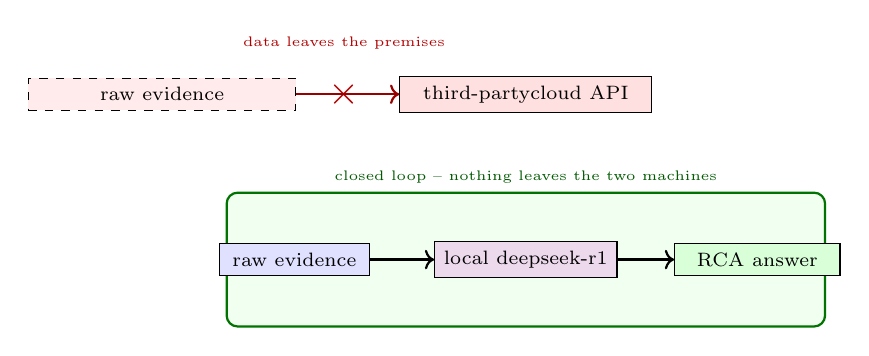
\begin{tikzpicture}[x=1.05cm,y=1cm, every node/.style={font=\scriptsize}]
    \node[draw, rectangle, fill=red!8, dashed, minimum width=3.4cm] (evd) at (0,2.6) {raw evidence};
    \node[draw, rectangle, fill=red!12, minimum width=3.2cm] (cloud) at (4.4,2.6) {third-party\\cloud API};
    \node[font=\Large, red!70!black] at (2.2,2.6) {$\times$};
    \draw[->, thick, red!60!black] (evd) -- (cloud);
    \node[font=\tiny, red!70!black] at (2.2,3.25) {data leaves the premises};
    \node[draw, rounded corners, thick, green!45!black, fill=green!6, minimum width=7.6cm, minimum height=1.7cm] (loop) at (4.4,0.5) {};
    \node[draw, rectangle, fill=blue!12, minimum width=1.9cm] (evd2) at (1.6,0.5) {raw evidence};
    \node[draw, rectangle, fill=violet!15, minimum width=2.3cm] (llm) at (4.4,0.5) {local deepseek-r1};
    \node[draw, rectangle, fill=green!15, minimum width=2.1cm] (ans2) at (7.2,0.5) {RCA answer};
    \draw[->, thick] (evd2) -- (llm);
    \draw[->, thick] (llm) -- (ans2);
    \node[font=\tiny, green!35!black] at (4.4,1.55) {closed loop -- nothing leaves the two machines};
\end{tikzpicture}
\end{adjustbox}
\vspace{0.2cm}
\begin{alertblock}{The Core Principle}
\centering\small A local, open-weight model running entirely offline on our own machines is the only way to get full control over both the data \emph{and} the model itself.
\end{alertblock}
\end{frame}

\begin{frame}{The Sovereign AI Stack}
\slidepurpose{Show every layer of the stack under direct control}{Data sovereignty}
\centering
\begin{adjustbox}{max width=0.9\linewidth, max height=0.44\textheight}
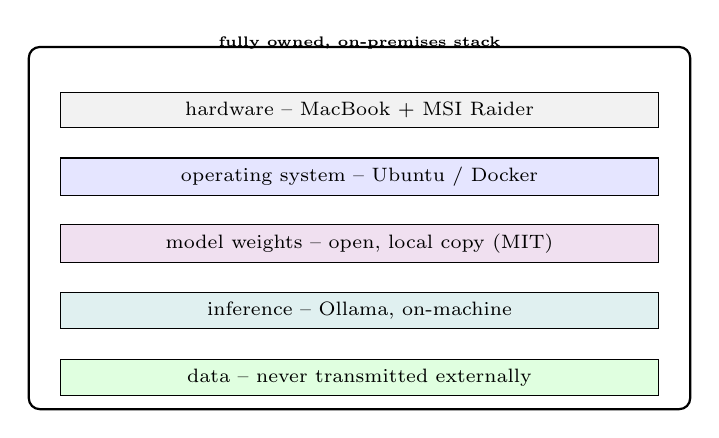
\begin{tikzpicture}[x=1cm,y=1cm, every node/.style={font=\scriptsize}]
    \node[draw, thick, rounded corners, minimum width=8.4cm, minimum height=4.6cm] (box) at (4.2,2.2) {};
    \node[font=\bfseries\tiny] at (4.2,4.55) {fully owned, on-premises stack};
    \node[draw, rectangle, fill=gray!10, minimum width=7.6cm] at (4.2,3.7) {hardware -- MacBook + MSI Raider};
    \node[draw, rectangle, fill=blue!10, minimum width=7.6cm] at (4.2,2.85) {operating system -- Ubuntu / Docker};
    \node[draw, rectangle, fill=violet!12, minimum width=7.6cm] at (4.2,2.0) {model weights -- open, local copy (MIT)};
    \node[draw, rectangle, fill=teal!12, minimum width=7.6cm] at (4.2,1.15) {inference -- Ollama, on-machine};
    \node[draw, rectangle, fill=green!12, minimum width=7.6cm] at (4.2,0.3) {data -- never transmitted externally};
\end{tikzpicture}
\end{adjustbox}
\vspace{0.15cm}
{\footnotesize
\begin{itemize}
    \item Every layer of the stack is under direct organizational control.
    \item No vendor lock-in, no per-token cost, no data-residency ambiguity.
    \item Compliance by construction -- not by contract or by trust.
\end{itemize}}
\end{frame}

\begin{frame}{Current Status: Proof of Concept}
\slidepurpose{Position what is delivered today against what comes next}{Closure -- PoC status}
\centering
\begin{adjustbox}{max width=0.96\linewidth, max height=0.40\textheight}
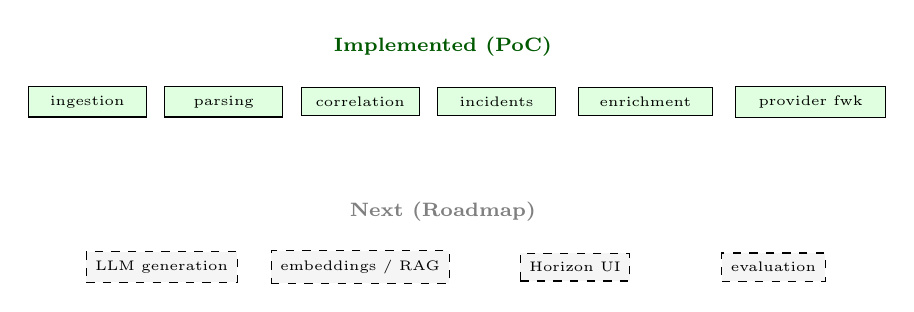
\begin{tikzpicture}[x=1.05cm,y=1cm, every node/.style={font=\tiny}]
    \node[font=\bfseries\scriptsize, green!35!black] at (4.3,3.0) {Implemented (PoC)};
    \node[draw, rectangle, fill=green!12, minimum width=1.5cm] at (0,2.3) {ingestion};
    \node[draw, rectangle, fill=green!12, minimum width=1.5cm] at (1.65,2.3) {parsing};
    \node[draw, rectangle, fill=green!12, minimum width=1.5cm] at (3.3,2.3) {correlation};
    \node[draw, rectangle, fill=green!12, minimum width=1.5cm] at (4.95,2.3) {incidents};
    \node[draw, rectangle, fill=green!12, minimum width=1.7cm] at (6.75,2.3) {enrichment};
    \node[draw, rectangle, fill=green!12, minimum width=1.9cm] at (8.75,2.3) {provider fwk};
    \node[font=\bfseries\scriptsize, gray] at (4.3,0.9) {Next (Roadmap)};
    \node[draw, rectangle, dashed, fill=gray!8] at (0.9,0.2) {LLM generation};
    \node[draw, rectangle, dashed, fill=gray!8] at (3.3,0.2) {embeddings / RAG};
    \node[draw, rectangle, dashed, fill=gray!8] at (5.9,0.2) {Horizon UI};
    \node[draw, rectangle, dashed, fill=gray!8] at (8.3,0.2) {evaluation};
\end{tikzpicture}
\end{adjustbox}
\vspace{0.15cm}
{\footnotesize
\begin{itemize}
    \item This is a \textbf{PoC}: ingest $\to$ parse $\to$ correlate $\to$ detect $\to$ enrich is implemented and tested end to end.
    \item Provider framework (config, security, activation) is already built -- ready to plug in Ollama.
    \item Next: wire live \texttt{deepseek-r1:8b} generation, then retrieval, then the Horizon UI.
\end{itemize}}
\end{frame}

\begin{frame}{Conclusion}
\slidepurpose{Close on the core value proposition}{Closure}
\begin{alertblock}{Key Takeaway}
    The OpenStack RCA Copilot turns scattered, cross-service logs into a bounded, explainable incident graph -- reasoned over by a model that never leaves the building. The evidence pipeline is implemented and tested; the AI layer is the next milestone.
\end{alertblock}
\centering
\vspace{0.4cm}
\Large Thank you --- Questions?
\end{frame}

\end{document}